\documentclass[]{subfiles}

\begin{document}
\section{Anforderungen}
    Im folgenden Abschnitt werden die Anforderungen an ein Netzwerk-Test-System formuliert.
    Es werden die Kern-Akteuere identifiziert und deren Funktion und Abhängigkeiten 
    und Anforderungen formuliert, um auf dieser Basis die Software zu entwerfen.
    
    \subsection{Akteure in einem Netzwerksystem}
    In der Praxis gibt es für die verschiedenen Akteure in einem Netzwerksystem
    unterschiedliche Bezeichnungen. Beispielsweise ist oft nicht klar, was der 
    Unterschied zwischen einem Netzwerk-Architekten und einem Netzwerk-Engineer
    ist und welche Verantwortungen diese nun genau haben. Wir haben eine eigene
    Unterscheidung der Akteure formuliert und diese in den kommenden Sektionen
    dokumentiert, um eine einheitliche Basis für die Leser zu schaffen.

    \subsubsection*{Netzwerk-Architekt}
    Ein Netzwerk-Architekt plant und erstellt Kommunikationsnetzwerke.
    Im Zuge dieser Arbeit wurde zwischen dem Architekten als verantwortlichen
    Senior-Network-Engineer und einem Network Engineer (Junior oder Senior)
    als operativen Mitarbeiter unterschieden. 
    Der Architekt nimmt dabei eher die Rolle des Managers oder Teamleiters ein. 
    Er führt dabei normalerweise keine Konfigurationen am Netzwerk durch.

    \subsubsection*{Netzwerk-Engineer}
    Ein Netzwerk-Engineer ist für die Installation und Instandhaltung 
    eines Netzwerks zuständig. 
    Er ist dem Netzwerk-Architekten unterstellt und setzt mit Ihm
    zusammen die geplanten Arbeiten um. 

    \subsubsection*{Netzwerk-Administrator}
    er Netzwerk Administrator hat üblicherweise eine abgeschlossene Berufslehre 
    in der Informatik und arbeitet zusammen mit dem Netzwerk-Engineer am Netzwerk. 
    Es wird davon ausgegangen, dass ein Netzwerk Administrator keine bis wenige 
    Programmierkenntnisse hat. 
    Ein Netzwerk Administrator hat, je nach Grösse des Netzwerks, 
    nur Kenntnisse über einen Teil der Netzwerkumgebung. 
    Er führt dabei ihm vom Architekten oder Engineer vorgegebene Arbeiten 
    aus und muss dazu nicht den vollen Überblick über das Netzwerk und die 
    darin verwendeten Technologien haben.

    \subsubsection*{Netzwerk-User}
    Benutzer der Netzwerkumgebung. User können das Netzwerk verwenden,
    aber nicht dessen Konfigurationen anpassen.


    \subsubsection*{Netzwerk-Gerät}
    Ein Netzwerkgerät kann aus Hardware wie Switch, Router oder Server
    bestehen oder Virtuell als Software implementiert sein. 
    Im Zuge der Arbeit werden Netzwerkgeräte auch als Netzwerk-Devices 
    oder einfach Device bezeichnet. 
    Typischerweise haben Devices eine Statische Konfiguration und einen 
    dynamischen Zustand zur Laufzeit. 
    In den kommenden Kapiteln wird genauer auf Netzwerkgeräte eingegangen.

    \subsubsection*{Netzwerk-Verbindung}
    Die Netzwerkverbindung ist der Kommunikationskanal zwischen den einzelnen
    Netzwerkgeräten. Sie kann in physischer Form als Kabel, oder mit kabellosen
    Mitteln z.B. Funk umgesetzt sein. Die Wahl des Übertragungsmediums hat
    grossen Einfluss über die verfügbare Bandbreite und mögliche Störfaktoren.

    \subsubsection*{Repository/Inventar}
    Im Inventar werden die Unterschiedlichen Devices mit den für den 
    Betrieb wichtigsten Parametern gespeichert. 
    Das Inventar kann in digitaler Form als Repository, 
    als File auf einem Ordner/Computer, 
    oder analogin einem Dokumentenorder abgelegt sein. 
    Das Inventar wird benötigt, um die aktuellen Konfigurationen, 
    die physische Position des Geräts oder sonstige für den Betrieb 
    relevanten Informationen zu dokumentieren.

    \newpage

    \subsection{Akteure in der zu entwickelnden Software}

    \subsubsection*{Testprogramm}
    Das Testprogramm ist der Kern des zu entwickelnden Systems dieser Arbeit.
    Es Interagiert mit den anderen Akteuren und hat, vom Akteur und Kontext abhängig, 
    unterschiedliche Anforderungen.
    Es soll so aufgebaut sein, dass ein Benutzer der Software diese mit möglichst 
    geringem Aufwand bedienen kann.


    \subsubsection*{Testdefinitionssprache}
    Wird im Rahmen dieser Arbeit auch als Testbeschreibungssprache oder Definitionssprache
    bezeichnet. Eine Testdefinition beschreibt die einzelnen Testfälle, die von einem
    System durchgeführt werden sollen.
    Die Definitionssprache soll dabei in einem Format gehalten werden, das von 
    allen Benutzern der Software verstanden wird und von diesen erweitert werden kann.

    \subsubsection*{Testreport}
    Ein Testreport soll, möglichst einfach und genau, die Ergebnisse eines 
    Netzwerktests aufzeigen. 
    Fehlgeschlagene Tests sollen dabei möglichst einfach und schnell zu erkennen
    sein und alle Informationen beinhalten, die ein Betrachter benötigt, um
    den Fehler im System zu lokalisieren und beheben.
    Ausserdem muss mindestens noch ein Zeitstempel vorhanden sein, um die
    Historie vergangener Netzwerktests nachvolziehen zu können.
    Testreporte können auf dem System, welches die Tests ausführt, oder in 
    einem zentralen Repository abgelegt werden, damit mehrere Mitglieder eines 
    Netzwerkteams gleichzeitig darauf zugreifen können.     

    \subsubsection*{Kommunikationskanal}
    Der Kommunikationskanal, nicht zu verwechseln mit der Netzwerkverbindung zwischen
    zwei Netzwerkgeräten, verbindet ein zu testendes Netzwerk mit dem Testprogramm.
    Möglichkeiten für einen Kanal sind beispielsweise das SSH (secure shell) Protokoll
    oder der Restconf Standard.
    Dies kann über eine Kabelverbindung oder Kabellos geschehen.
    Die Wahl des Kommunikationskanals beeinflusst dabei, in welcher Form 
    Netzwerktests durchgeführt werden können und in welchem Format die Ergebnisse 
    zurückgegeben werden.

    \subsubsection*{Netzwerktest}
    Werden heute meist manuell oder mit Hilfe eines Skripts durchgeführt.
    Ein automatisierter Netzwerktest sollte hypothetisch ad-hoc nach jeder
    Konfigurationsänderung vom Testprogramm durchgeführt werden um 
    die Funktionsweise des Netzwerks zu validieren. 
    Ein Benutzer des zu entwickelnden Systems soll in der Lage sein, 
    mit nur geringer Einarbeitungszeit, Netzwerktests zu spezifizieren und
    durchzuführen.

    \subsection{Use Cases}
    \subsubsection{Use Case Diagramm}
    \begin{figure}[!h] 
        \centering
        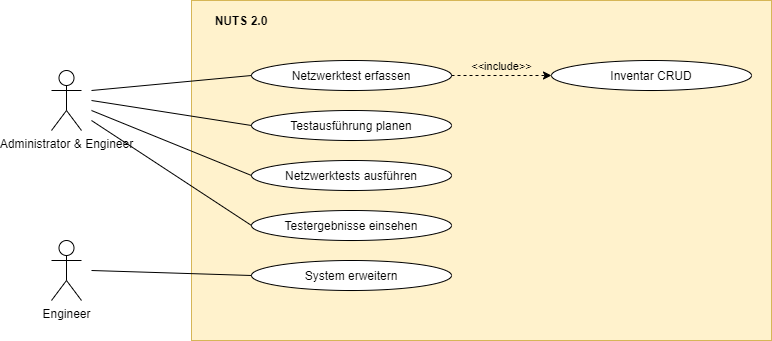
\includegraphics[scale=0.6]{../../99_Vorlagen/Bilder/UseCaseDiagram.png}
        \caption{Use Case Diagramm}
    \end{figure}
    \subsubsection{Aktoren}
    Die Primären Akteure sind der Netzwerk Architekt, -Administrator und -Engineer. 
    Der Architekt will primär die Ergebnisse einsehen können, um zu sehen, dass
    das Netzwerk korrekt funktioniert. 
    Ausserdem möchte er, beispielsweise um eine Erweiterung des Netzwerks zu 
    Planen, eine Ausführung von Netzwerktests konfigurieren und durchführen.
    Der Administrator will Netzwerktests erfassen, deren Durchführung planen, 
    die Tests durchführen und die Ergebnisse einsehen.
    Der Engineer möchte neben den Tätigkeiten, die der Administrator ausführt,
    zudem das Testsystem um weitere Netzwerktests erweitern können.

    \subsection{Beschreibung Usecases (Brief)}

        \paragraph{Netzwerktest erfassen}

        \paragraph{Inventar CRUD}

        \paragraph{Testdurchführung planen}

        \paragraph{Netzwerktests durchführen}

        \paragraph{Testergebnisse einsehen}

        \paragraph{System erweitern}



\end{document}